\begin{titlepage}
  \newgeometry{margin=0pt}
  
  \begin{tikzpicture}[remember picture, overlay]
  
    % Background photo cropped to the cover area without distortion
    \node[anchor=center, inner sep=0pt] at ([yshift=1in]current page.center) {%
      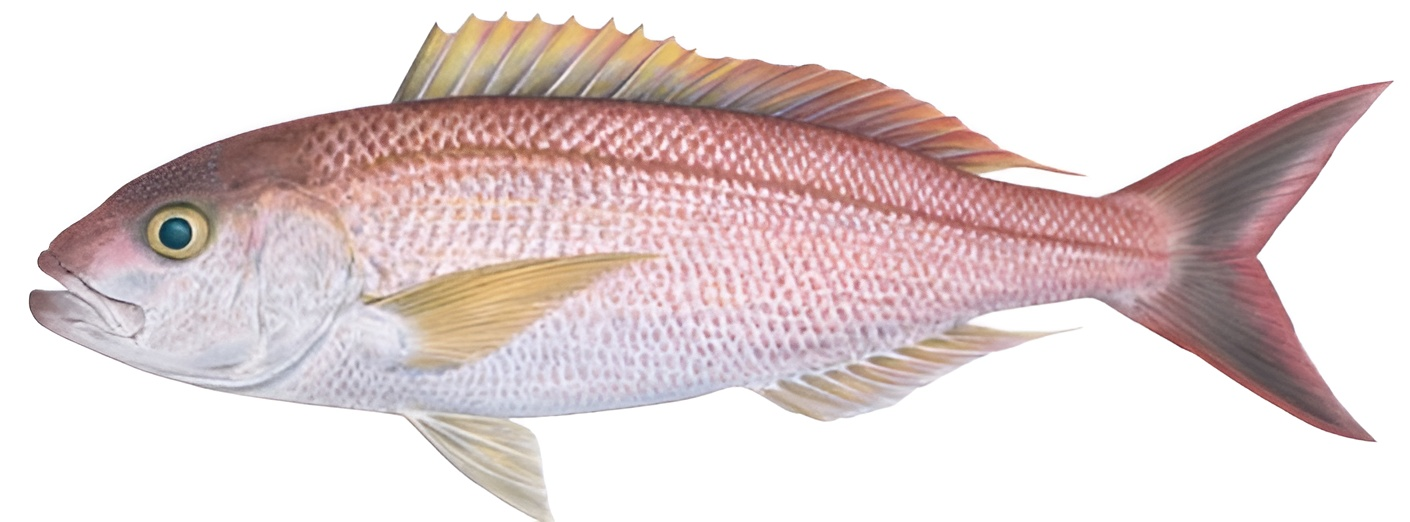
\includegraphics[width=1\paperwidth, height=0.55\paperheight, keepaspectratio, clip]{P_filamentosus.png}%
    };
    
   % NOAA logo - top left corner, full bleed
    \node[anchor=north west, inner sep=0pt] at (current page.north west) {%
      
\includegraphics[height=5.07in]{NOAA_corner_logo.png}%
    };
    
    % Navy footer bar at bottom
    \fill[noaanavy]
      (current page.south west) rectangle ++(\paperwidth, 3.5cm);
      
    % Footer text (white)
    \node[anchor=south west, text=white, inner sep=12pt, align=left,
          font=\small] at (current page.south west) {%
      NOAA Technical Memorandum NMFS-PIFSC-???\\
      U.S. Department of Commerce\\
      National Oceanic and Atmospheric Administration\\
      National Marine Fisheries Service\\
      Pacific Islands Fisheries Science Center\\
      \today
    };
    
  \end{tikzpicture}

  % Title and author text
  \vspace*{0.6\paperheight}
  \hspace{1cm}
  \begin{minipage}{0.85\textwidth}
    {\fontspec{Arial Narrow Bold}\fontsize{26pt}{30pt}\selectfont Optimizing Fishery-Independent Surveys: Evaluating Sampling Effort for the Hawaiian 'Ōpakapaka Stock Assessment \par}
    \vspace{2cm}
    {\normalsize Megumi Oshima, Marc Nadon, John Syslo, Hongguang Ma, and Felipe Carvalho\par}
  \end{minipage}
  \vfill

\end{titlepage}
\restoregeometry

% --- About/Title page ---
\clearpage
\thispagestyle{fancy}
\setcounter{page}{2}    % <--- FORCE LATEX TO LOG THIS AS PAGE 2 (Overrides cover page reset)
\vspace*{1cm}

{\fontspec{Arial Narrow Bold}\fontsize{26pt}{30pt}\selectfont Optimizing Fishery-Independent Surveys: Evaluating Sampling Effort for the Hawaiian 'Ōpakapaka Stock Assessment\par}
\vspace{1cm}

{\normalsize Megumi Oshima, Marc Nadon, John Syslo, Hongguang Ma, and Felipe Carvalho\par}
\vspace{1cm}

{\small
Pacific Islands Fisheries Science Center\\
National Marine Fisheries Service\\
1845 Wasp Boulevard\\
Honolulu, HI 96818

}



\vspace{1cm}

% Green highlight box
% Technical Memorandum Series Number Block (No Highlight)
\parbox{\textwidth}{%
  \small NOAA Technical Memorandum NMFS-PIFSC-\#\#\#\\
  {[Month]} {[Year]}
}

\vspace{1cm}


\includegraphics[width=1.3in]{900px-Seal_of_the_US_DoC.png}

\vspace{0.5cm}

{\small
U.S. Department of Commerce\\
National Oceanic and Atmospheric Administration\\
National Marine Fisheries Service\\
Pacific Islands Fisheries Science Center
}

\clearpage


%Acknowledgements
\clearpage
\thispagestyle{empty}   % <--- COMPLETELY REMOVES FOOTERS & NUMBERS FROM ACKNOWLEDGEMENTS

\vspace*{1cm}

{\fontspec{Arial Bold}\fontsize{14pt}{16pt}\selectfont Acknowledgements\par}
\vspace{0.5cm}

{\fontspec{Arial}\fontsize{12pt}{14pt}\selectfont \par}
\vspace{0.25cm}

{\fontspec{Arial}\fontsize{12pt}{14pt}\selectfont Cover drawing: Hawaiian 'Ōpakapaka \fontspec{Arial Italic}\fontsize{12pt}{14pt}\selectfont(Pristipomoides filamentosus) \fontspec{Arial}\fontsize{12pt}{14pt}\selectfont. Drawing credit: Hawai'i Division of Aquatic Resources. Artist: Les Hata.\par}
\vspace{0.25cm}

{\fontspec{Arial}\fontsize{12pt}{14pt}\selectfont Edited by --------------.\par}
\vspace{0.5cm}


{\fontspec{Arial Bold}\fontsize{14pt}{16pt}\selectfont Recommended citation\par}
\vspace{0.25cm}

{\fontspec{Arial}\fontsize{12pt}{14pt}\selectfont Oshima, M., Nadon, M., Syslo, J., Ma, H., \& Carvalho, F. (2026). Optimizing fishery-independent surveys: Evaluating sampling effort for the Hawaiian 'Ōpakapaka stock assessment (Technical Memorandum Series, TM-PIFSC-???). Pacific Islands Fisheries Science Center.\par}
\vspace{0.5cm}

{\fontspec{Arial Bold}\fontsize{14pt}{16pt}\selectfont Copies of this report are available from\par}
\vspace{0.25cm}

{\fontspec{Arial}\fontsize{12pt}{14pt}\selectfont
Pacific Islands Fisheries Science Center\\
National Marine Fisheries Service\\
National Oceanic and Atmospheric Administration\\
1845 Wasp Boulevard, Building \#176\\
Honolulu, Hawaiʻi 96818\par}
\vspace{0.5cm}


% --- Switch to Roman numerals for front matter ---
%\clearpage
%\pagenumbering{roman}

{\fontspec{Arial Bold}\fontsize{14pt}{16pt}\selectfont Or online at\par}
\vspace{0.25cm}

{\fontspec{Arial}\fontsize{12pt}{14pt}\selectfont \href{https://repository.library.noaa.gov/}{\color{blue}\underline{https://repository.library.noaa.gov/}}\par}


% --- Switch to Roman numerals for the Table of Contents page ---
\clearpage
\pagenumbering{roman}   % <--- FORCES THE TOC PAGE TO START FRESH AT ROMAN 'i'
